\documentclass[11pt]{article}
\usepackage{geometry}
\usepackage{graphicx}
\usepackage{svg}
\geometry{a4paper, 
          total={17cm, 24cm}, 
          left=2cm, 
          top=1.5cm,
          bottom=1.5cm,}


\title{\textbf{Výstupná správa\\1. časť projektu INC}}
\author{\textbf{meno:} Katarína Mečiarová \hspace{2.3cm} \textbf{login:} xmeciak00}\date{}

\begin{document}

\maketitle

\section{Architektúra navrhnutého obvodu (na úrovni RTL)} 
\subsection{Schéma obvodu}
\begin{figure}[here]
    \centering
    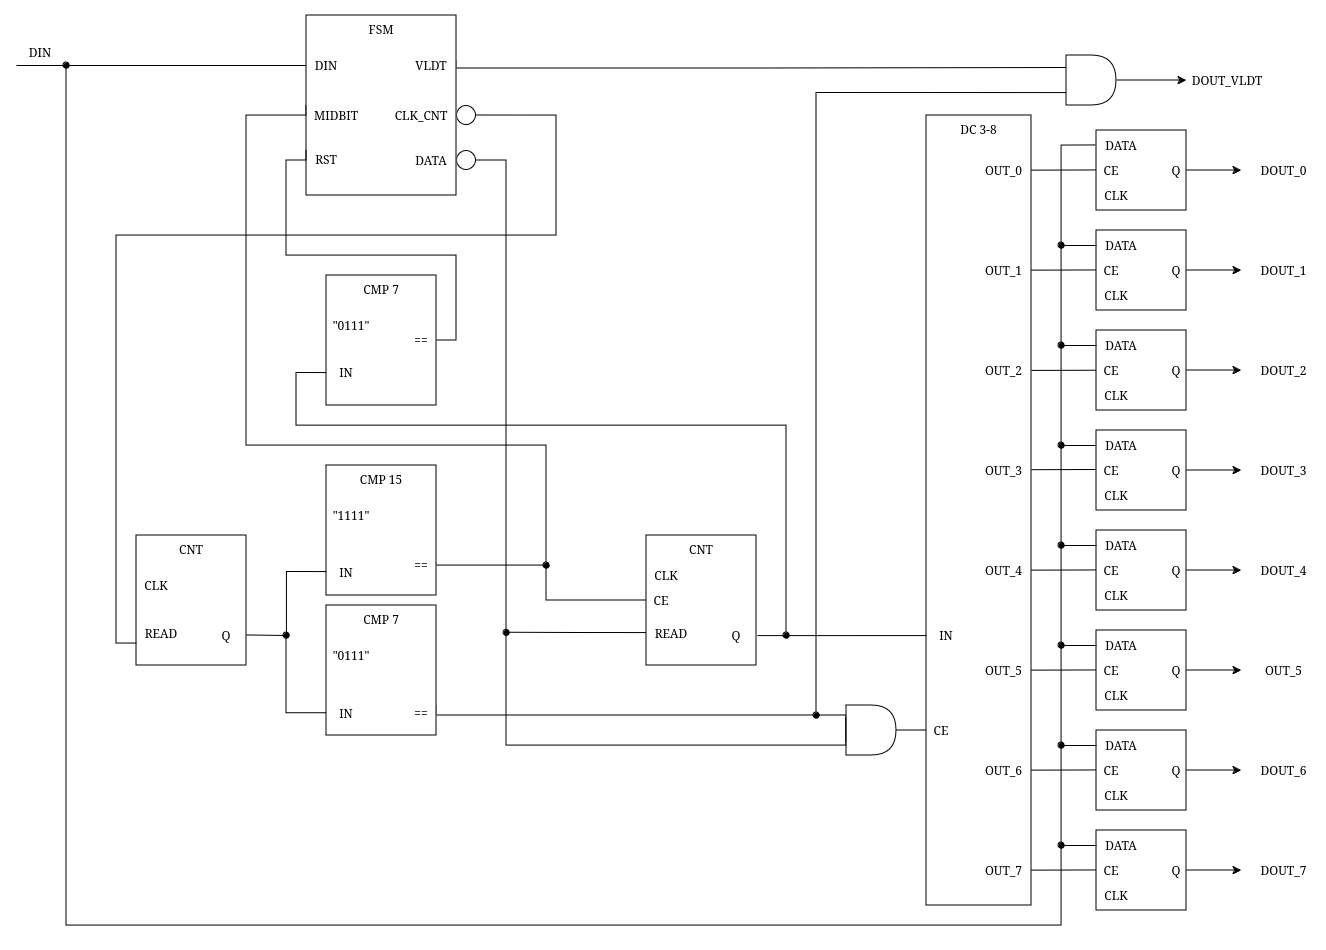
\includegraphics[width=1\textwidth]{OBVOD.png} % zmena šírky na 100% šírky textu
    Poznámka: CLK a stabilné vstupy ako napr."0111" zapisujeme, ale nevyznačujeme.
\end{figure}

\subsection{Popis}
Pokým je na CLK\_CNT  '0', obvod nič (okrem resetu) nevykonáva. Keď sa cez CLK\_CNT pošle '1', teda READ prvého (zľava) CNT dostáva '0' (negácia), začne počítať.
Počítam osobitne MIDBIT aj celý BIT. 
Jeden bit trvá 16 jednotiek CLK (ďalej tikov), teda MIDBIT sa nachádza v každej polovici 16 tikov - po prvých siedmych začínam čítať a následne pokračujem po každom pätnástom tiku. 
Čítať znamená, že povolím zápis DIN do konkrétneho registra, ktorý určujem druhým CNT - keď sa výstup prvého CNT rovná "1111" resp. "15", druhé CNT sa inkrementuje a taktiež sa odosiela informácia na FSM ako signál MIDBITu. 
Ak druhý CNT inkrementoval už 7 krát a CMP 7 vyhodnotí zhodu s "0111", očakávam STOPBIT, čítanie aj počítanie sa ukončuje - na vstup RST sa odosiela informácia v podobe jednotky, následne sa na CLK\_CNT odosiela '0' a kruh sa uzatvára. Čakám na ďalší STARTBIT.

\section{Návrh automatu (FSM)}
\subsection{Schéma automatu}
Legenda:\\
- stavy: IDLE, START, DATA, STOP\\
- vstupy: DIN, MIDBIT, RST\\
- Moorove výstupy: VLDT, DATA, CLK\_CNT\\
\begin{figure}[here]
    \centering
    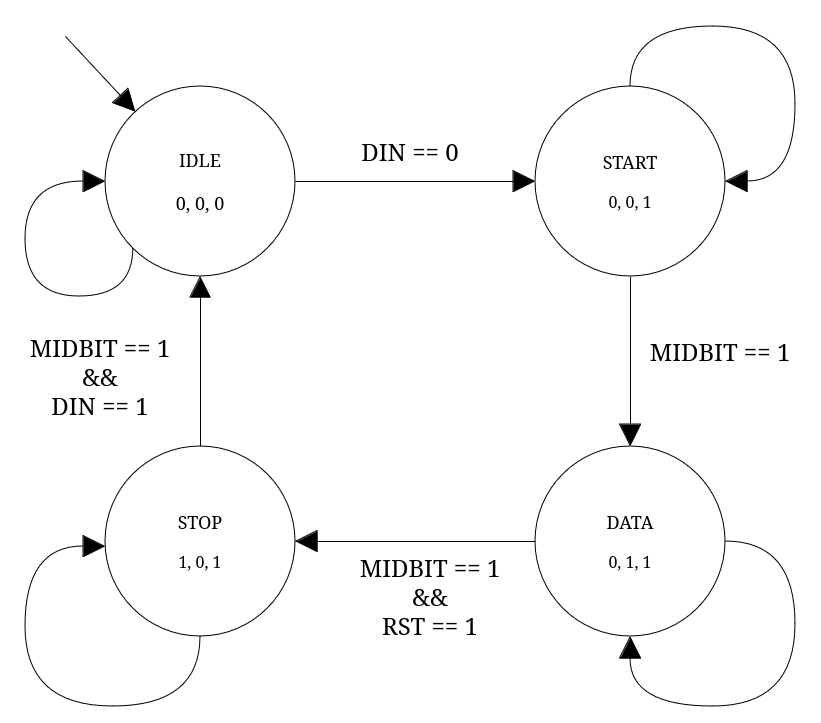
\includegraphics[width=0.7\textwidth]{automat.png} % zmena šírky na 70% šírky textu
\end{figure}

\subsection{Popis}
Stav IDLE - čaká na vstup DIN, ak je DIN rovné '0', prechádza do stavu START.\\
Tj. ak je DIN rovné '0', nastavuje sa CLK\_CNT na '1' a počíta sa do '7' al. '111', kým sa nenastavuje MIDBIT na '1'.\\
Stav DATA - ak je MIDBIT rovné '1', nastavuje sa DATA na '1' a počíta sa do '7' al. '111', kým sa nenastavuje RST na '1'\\
Stav STOP - ak je RST rovné '1', nastavuje sa DATA na '0' a prechádza sa do stavu IDLE, kde znova čakáme na nový STARTBIN al. DIN=0.\\



\end{document}
